%!TEX root=../documentation-bachlorthesis-speicherarchitektur-lstucker.tex

\cleardoublepage
\chapter{Ist-Analyse}
Ziel der Ist-Analyse ist es, mit der Situationsanalyse den aktuellen Stand des bestehenden Systems bzw. der Speicherinfrastruktur zu beschreiben und zu bewerten. Die Ist-Analyse ist Ausgangspunkt für das Soll-Konzept und dient zur Darstellung der Vor- und Nachteile zwischen den beiden Systemen. Allerdings fehlen vom bisherigen System historische Messdaten, welche nicht mehr eruiert werden konnten.
Die Angaben für die Ist-Analyse wurden in diversen Interviews mit dem Auftraggeber und aus den von ihm gelieferten schriftlichen Dokumenten erhoben und zusammengestellt. 

\section{Bestandesaufnahme}
\subsection{Anwendungs-Architektur}
Die genaue Anwendungs-Architektur wird hier nicht beschrieben, da dies die Geschäftsgeheimnisse des Auftraggebers verletzen würde. Es werden deshalb nur die Teile davon beschrieben, welche die Geschäftsgeheimnisse des Auftraggebers nicht verletzen und für diese Arbeit von Belang sind.

Die Applikation ist eine Web-Applikation, welche auf dem Web-Framework Ruby On Rails aufsetzt.
Wie dem Namen "'Ruby On Rails"' zu entnehmen ist, basiert das Framework auf der Programmiersprache Ruby. Ruby ist eine dynamische, Objekt-orientierte, interpretierbare Programmiersprache, von Yukihiro Matsumoto, der sie 1995 der Öffentlichkeit vorgestellt hat und heute sehr beliebt ist und sich einer breiten Gemeinschaft (engl. Community) erfreut. Ein Ruby Programm benötigt für deren Ausführung keine Kompilation.

Ruby On Rails auch "'Rails"' oder "'RoR"' genannt, implementiert eine Model-View-Controller Architektur. Die drei Sub-Frameworks, spielen dabei eine signifikante Rolle in der Separierung des Codes: Active Record, Action View, und Action Controller. Die drei Sub-Frameworks sind auch im refabb{abb:Rails-Architektur} dargestellt (nach \cite{Bachle2007}).

\begin{center}
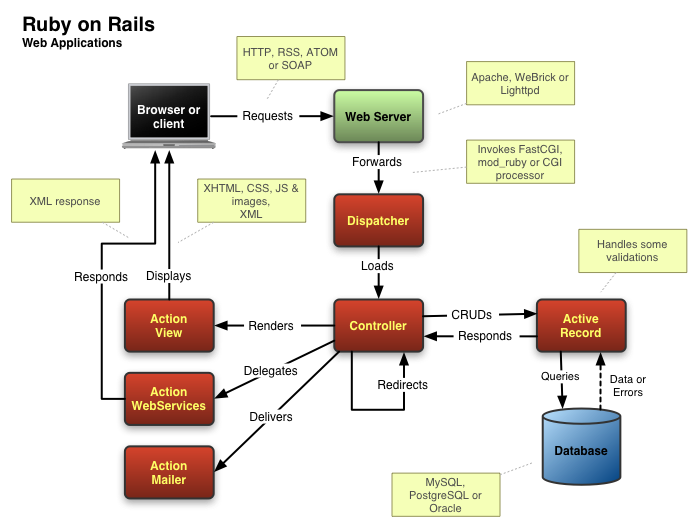
\includegraphics[width=\linewidth, keepaspectratio = true]{media/rails-architecture.png}
\mycaption{figure}{\label{abb:Rails-architektur}Rails Architektur \cite{Niwatori2008}}
\end{center}

Beides, Ruby On Rails und Ruby sind Open-Source Programme. Die Quellprogramme sind für jeden Programmierer offen. Ruby wird unter der Lizenz "'Ruby License"' und GPL veröffentlicht, während Rails unter der "'MIT License"' veröffentlicht ist.

\subsection{System-Architektur}\label{System-Architektur}
Die bestehende Kunden-System-Architektur besteht aus einem einzelnen Server, welcher von einem bekannten deutschen Webhosting-Provider gemietet wird. Beim gemieteten System handelt es sich um einen x64 Mikroarchitektur.

\subsection{Speicher-Architektur}
Die Speicher-Architektur besteht aus einem internen Block-basierendem RAID-5 Festplattenspeicher. Die im Server verbauten Festplatten (RAID-5) werden mittels dem Linux Software RAID Kernel\footnote{\url{https://raid.wiki.kernel.org/}} und dem Verwaltungstool mdadm\footnote{\url{http://neil.brown.name/blog/mdadm}} zu einer logischen Einheit zusammengefasst. Für das RAID-5 werden drei "'SATA 2"' Festplatten verwendet, welche jeweils eine Speicherkapazität von 2 Terabyte bzw. 1.818 Tebibyte aufweisen.

Im RAID Speicher sind ein root Dateisystem für das Betriebsystem, die Webapplikation, Datenbank, Logdateien und sämtliche Bilddaten installiert.

\subsection{Speicherkapazität}
Die von RAID-5 zur Verfügung gestellte Speicherkapazität beträgt gemäss \refeqlb{eqn:RAID-5-3disk} 3.636 Tebibyte, davon sind nach Installation des Dateisystems $\approx 3.5$ Tebibyte bzw. ca. 3.8 Terabyte effektiv verfügbar. Davon sind anhand des \textit{df}\footnote{\url{http://www.debianadmin.com/manpages/dfmanpage.htm}}
 Befehls, wie im \reflisting{df} ersichtlich, ca. 2.5 Terabyte für das Betriebsystem, die Webapplikation, Datenbank, Logdateien und Bilddaten reserviert. Als freier Speicherplatz verbleiben ca. 1.3 Terabyte.

\begin{equation}
\mbox{Speicherkapazität RAID-5}= (3 - 1) * 1.818 \, \mathrm{TiB} = 3.636 \, \mathrm{TiB}
\label{eqn:RAID-5-3disk}
\end{equation}

\begin{lstlisting}[label=df, language=Bash, caption=Report Dateisystem Speicherplatz Belegung in Dezimal Prefix ]
root@www1:~# df -h
Filesystem            Size  Used Avail Use% Mounted on
simfs                      3.8T  2.5T  1.3T   67% /
\end{lstlisting}

\subsection{Datenwachstum}
Das \refabb{abb:disk-usage-by-year} zeigt den Speicherzuwachs von Mitte Juni bis Ende November 2011.

\begin{center}
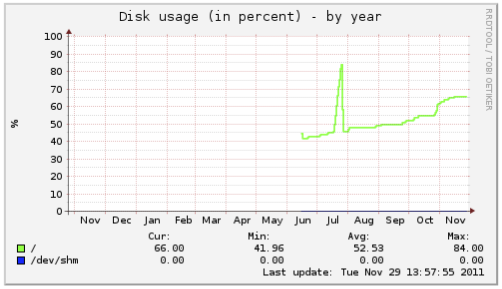
\includegraphics[width=\linewidth, keepaspectratio = true]{media/disk-usage-by-year.png}
\mycaption{figure}{\label{abb:disk-usage-by-year}Verhältnis von Speicheplatzverbrauch zur Speicherkapazität in Prozent in einer Zeitspanne von einem Jahr}
\end{center}

\subsection{Zugriffswachstum}
Für die Ist-Aufnahme konnten keine historischen Messdaten zur Verfügung gestellt werden.

\subsection{Skalierbarkeit Datenvolumen}
Während dem Betrieb ist ein Ausbau der Speicherkapazität (Skalierbarkeit) nicht möglich. Eine Vergrösserung der Speicherkapazität ist nur durch den Wechsel auf ein anderes Hostingprodukt möglich. Dies erfordert eine Migration auf eine neue Server-Plattform. 

\subsection{Skalierbarkeit Datenzugriffe}
Keine Skalierung möglich. 

\subsection{Daten Durchsatz I/O}
Für die Ist-Aufnahme konnten keine historische Messdaten zur Verfügung gestellt werden.

\subsection{Daten Redundanz}

Die Daten-Redundanz wird durch das RAID-5 gewährleistet.

\subsection{Datenverfügbarkeit}
Stromausfälle und Netzwerkstörungen im Rechenzentrum des \gls{Hosting} \gls{Provider}s führten zu Störungen und Ausfällen in der Webapplikation und in der Datenauslieferung. Die Störungen wurden jedoch nicht dokumentiert, weshalb keine statistische messbare Aussage über die erreichte Datenverfügbarkeit gemacht werden kann.

\subsection{Daten Sicherheit}
Die Daten sind durch Verschlüsselung vom unerlaubten Fremdzugriff geschützt. Für die Verschlüsselung wird das Device Mapper Module dm-crypt eingesetzt. dm-crypt verschlüsselt die Daten bereits auf Blockebene und ist somit für das Dateisystem transparent.
Der Hosting-Provider hat geeignete Objetkbezogene Schutzmassnahmen installiert, welche den unerlaubten physischen Zugriff auf die Systeme und Daten verhindert.

\subsection{Daten Integrität}
Zu jedem Bild wird eine Hash Prüfsumme (engl. Checksum) gespeichert, die bei jedem Backup geprüft wird. Die Daten-Integrität ist somit weitgehend sichergestellt.

\subsection{Sicherung}
Es wird täglich mittels dem Tool ccollect\footnote{\url{http://www.nico.schottelius.org/software/ccollect/}} ein R-Sync Sicherung (engl. Backup) der Daten erstellt. Die Sicherung wird ausser Hause gelagert.

\subsection{Wirtschaftlichkeit}
Die Kosten für die Speicherung der Daten inklusive Webinfrastruktur sind vergleichsweise zu alternativen Lösungen tief.

\subsection{Lokalität}

Die Web-Applikation inklusive dessen \gls{Primearen-Daten} werden am selben Standort betrieben. Die Sicherungsdaten (engl. Backupdata) werden an einen separaten Standort gelagert. Der Zugriff auf die Backup-Daten innert 30 Minuten ist gewährleistet.

\section{Analyse-Ergebnisse}

\subsection{System-Architektur}

\subsection{Datenwachstum und Speicherkapazität}
Die Messdaten aus dem \refabb{abb:disk-usage-by-year} zeigen, dass das Datenvolumen seit Juni 2011 bis Ende November 2011 mit Ausnahme einer unregelmässigen Spitze und einem grösseren Wachstumsschub Ende Oktober kontinuierlich zugenommen hat. Die etwas erhöhte Spitze lässt sich durch eine vorübergehende technische Änderung am System erklären und hat somit für die Auswertung keine Relevanz. Während der erwähnten Zeitspanne hat das Datenvolumen von 1,634 Terabyte auf 2,546 Terabyte zugenommen. Dies entspricht einer Datenzuwachsrate von 0,912 Terabyte bzw. 55,8\% in fünf Monate. Das durchschnittliche Datenwachstum beträgt 0,182 Terabyte bzw. 11,1\% pro Monat.

Setzt sich der bisherige Trend fort, so ist die verfügbare Speicherkapazität von 3,8 Terabyte in weniger als 7 Monate erschöpft. Berücksichtigt man bei diesem durchschnittlichen Datenwachstum mögliche Wachstumsschübe für Neukunden, welche durch das Einlesen von deren bestehende Bilddatenbanken entstehen könnten, so reduziert sich die Kapazitätsreserve nach unten und würde eine vorzeitige Umstellung auf ein neues System bedingen.

Gemäss des Auftraggebers ist ferner ein neues Feature für die Web-Applikation geplant, welches den Speicherplatzbedarf verdoppeln würde. Die aktuelle Speichersituation lässt momentan den produktiven Einsatz des neuen Feature nicht zu. Das durchschnittliche Datenwachstum würde voraussichtlich auf 0,364 Terabyte pro Monat steigen.

Die jetzige Speicherkapazität erfüllt schon heute die Anforderungen nicht mehr.

\begin{equation}
\mbox{Datenwachstum}_{Monate5} = 2,546 \mathrm{TB} - 1,634 \mathrm{TB} = 0,912 \mathrm{TB}
\label{eqn:Verfügbarkeit_5Monate}
\end{equation}

\begin{equation}
\mbox{Datenwachstum}_{Monate5} = \frac{0,912 \mathrm{TB}}{\frac{1,634 \mathrm{TB}}{100 \%}} = 55,813\%
\label{eqn:Verfügbarkeit_5Monate_in_Prozent}
\end{equation}

\begin{equation}
\mbox{Durchschnittliches Datenwachstum}_{Monate} = \frac{0,912 \mathrm{TB}}{5\mathrm{m}} = 0,1824 \mathrm{TB}
\label{eqn:Verfügbarkeit_1Monate}
\end{equation}

\begin{equation}
\mbox{Durchschnittliches Datenwachstum}_{Monate} = \frac{55,813\%}{5 \mathrm{m}} = 11,162\%
\label{eqn:Verfügbarkeit_1Monate_in_Prozent}
\end{equation}

\subsection{Skalierbarkeit Datenvolumen}\label{AnalyseSkalierbarkeitDatenvolumen}
Die eingesetzte Speicherarchitektur lässt eine Skalierung des Datenvolumen mittels hinzufügen von weiteren Festplatten oder durch Migration auf grössere Festplatten zu. Die maximale Anzahl von Festplatten wird dabei durch die Anzahl vorhandener SATA Anschlüsse im Server bestimmt. Beim eingesetzten Server handelt sich um ein Hostingprodukt, welches begrenzt ausbaubar ist. Bei Hostinglösungen erfolgt die notwendige Skalierung oft durch hochrüsten mittels Migration auf eine leistungsfähigere und besser ausgebaute Hostinglösung. Der Ausbau auf eine leistungsfähigere Hardware bedingt ferner die Prüfung und den allfälligen Ausbau des Service Levels Agreement. 

\subsection{Skalierbarkeit Datenzugriffe}
Eine mögliche Skalierung bezüglich des Datendurchsatzes könnte durch schnellere Festplatten, durch eine optimierte Verteilung der I/O-Operationen auf verschiedene Festplatten oder durch die Verteilung der Daten auf weitere Systeme erreicht werden. Zu beachten sind auch hier dieselben Prämissen, wonach wie beim Ausbau des Datenvolumens das bestehende System nur sehr begrenzt ausbaufähig ist bzw. auf ein anderes Hostingprodukt migriert werden müsste.

\textbf{Skalierung durch schnellere Festplatten:}
Moderne Festplatten, mit Ausnahme von den teuren Solid State Disk (SSD), bieten zwar eine grössere Speicherdichte, aber aufgrund der erreichten physikalischen Grenzen keine bedeutend effizientere IOPS. Eine Festplatte mit 7200 RPM erreicht durchschnittlich ein IOPS zwischen 75 und 100 IOPS. Bei SSD Disks wurden schon 1'190'000 IOPS in einem einzelnen PCI Geräte gemessen. \cite{Symantec2011} \cite{Fusionio} 
Ein Wechsel auf die genannten SSD Festplatten, ist momentan noch mit sehr hohen Kosten pro Gigabyte verbunden. Gartner geht davon aus, dass 2012 die Preise pro Gigabyte bei SSD auf durchschnittliche 1\$ sinken werden. Gegenüber den heutigen Preisen bei konventionellen Festplatten von 30 Cents pro Gigabyte ist dies immerhin 3x teurer. Aus diesem Grund werden SSD Disks bei grossen Datenvolumen meist noch nicht eingesetzt, ausser spezielle Anforderungen an die Performance rechtfertigt die höhere Investition. \cite{AgamShah2011}

\textbf{Skalierung duch Verteilung der I/O Operationen:}
Ein RAID oder Volume Manager bietet die Möglichkeit, die I/O Operationen auf mehrere Festplatten zu verteilen. In einem RAID-5 verkleinert sich wie in Kapitel \refchap{AnalyseSkalierbarkeitDatenvolumen} beschrieben, die MTTF mit jeder weiteren Festplatte. Zudem sind die verfügbaren Anschlüsse in einem Server ebenfalls ein zu berücksichtigender limitierender Faktor.

\textbf{Skalierung durch Verteilung der Daten:}
Beim Kunden haben nicht alle Kategorien von Daten dieselben Anforderungen an den Durchsatz. Datenbanken z.B. benötigen in der Regeln einen höheren IOPS als statische Daten wie z.B. Bild-Daten, welche weniger oft abgefragt werden. Für die Verteilung der Daten ist eine Änderung in der System-Architektur und allenfalls in der Anwendungs-Architektur sinnvoll. Ein Beispiel für eine solche Anpassung der System-Architektur wäre die Auslagerung der Datenbank auf ein separates System, welches mit schnellen Solid State Disk ausgerüstet ist. 

\subsection{Redundanz}
Eine RAID-5 System bietet wie im \refsec{RAID-5} beschrieben, keine 1:1 Redundanz. Die Daten sind im RAID-5 nicht doppelt gespeichert, sondern werden bei einen Datenverlust mittels XOR Operation aus den Parität Stripes und den vorhandenen Daten Stripe-Einheiten berechnet. 

Beim Zugriff auf einen verlorenen Daten Stripe werden die Daten online berechnet. Die Berechnung der Daten, verringert die Performance des Systems.

Treten bei einer Festplatte Fehler auf, werden die verlorenen Daten bei einem Zugriff aus der Parität Stripe Einheit berechnet. Der Zugriff auf die Daten ist somit während des Betriebs möglich. Wird die ausgefallen Festplatte durch eine neu intakte Festplatte ersetzt, können die Daten durch einen Wiederherstellungsprozess (engl. Rebuild) während des Betriebs wieder hergestellt werden, welcher je nach Datenvolumen mehrere Stunden oder Tage beanspruchen kann. Durch die Berechnung und Schreib/Lese Operationen im RAID während des Wiederherstellungprozesses verschlechtert sich der Datendurchsatz und I/O Rate für den Datenzugriff.

Einen Ausfall einer weiteren Festplatten kann das RAID-5 System nicht mehr kompensieren und führt zu einem physischen Datenverlust aller \gls{Primearen-Daten} . Die Daten müssen in der Folge mittels der Sicherung eingelesen und wiederhergestellt werden, was jedoch nur im Offline-Betrieb möglich ist. Während dieser Ausfallzeit (engl. Downtime) steht die Anwendung für den Benutzer nicht zur Verfügung, da diese Arbeit unplanmässig während den normalen Betriebsstunden durchgeführt werden müsste. Das Ausfallzeit könnte den Rahmen des vereinbarten SLAs mit dem Kunden sprengen. 

Bei Festplatten aus dem gleichen Produktionszyklus ist die Wahrscheinlichkeit eines zweiten Festplattenausfall signifikant höher als bei Festplatten aus unterschiedlichen Produktionszyklus.

\subsection{Service- und Daten-Verfügbarkeit}
Die bisherige System-Architektur ermöglicht keine AEC-2 Hochverfügbarkeit. Grund dafür ist die Fokussierung auf einen einzelnen Server in der Produktivumgebung. Der Server stellt eine "'Single Point of Failure"' (kurz SPOF) dar. Tritt beim Server eine Störung auf, wie sie zum Beispiel aufgrund eines Gerätedefektes oder bei Softwarefehlern auftreten können, kann der Service nicht von einem redundantem System übernommen oder weitergeführt werden. Eine Störung wird voraussichtlich die Verfügbarkeit während den Betriebszeiten stark gefährden und entspricht nicht den heutigen Anforderungen. Allfälliger SLAs gegenüber den Kunden könnten kaum eingehalten werden.

Die Netzwerkverfügbarkeit wird vom Hosting Anbieter gemäss den Allgemeinen Geschäftsbedingungen \cite{Ag2009} mit einer Verfügbarkeit von 99\% im Jahresmittel gewährleistet. Die Verfügbarkeit könnte somit bei einem 24x365 Stunden Betrieb während 87,6 Stunden nicht gewährleistet sein. Die max. Ausfallzeit (engl. Downtime) pro Ereignis oder Monat wäre zu untersuchen und mit dem Hostingprovider zu vereinbaren bzw. mit den SLAs gegenüber den Kunden in Einklang zu bringen.

Das Speichersystem für sich selbst betrachtet kann die Verfügbarkeit und die Daten-Integrität gewährleisten, sofern keine Störung durch einen Festplattendefekt eintritt. Das Speichersystem, welches ein interner Block-basierenden RAID-5 Speicher darstellt, ist ein Bestandteil des Serversystems und weist deshalb die selbe Verfügbarkeitsstufe wie das Serversystem auf. Die Service und Datenverfügbarkeit weist aus den genannten Gründen eine Verfügbarkeit Stufe von "'Highly Reliable"' AEC-1 auf.

Zudem werden die Daten und Applikation nur an einem einzigen Standort gehalten und betrieben. Treten externe, unvorhersehbare Ereignisse auf, wie z.B. ein lokaler Stromausfall, ein Gebäudebrand oder eine Naturkatastrophe, kann der Betrieb nicht ohne die Wiederherstellung des ganzen Systems (neue Hardware und Rückspielung der Daten vom der Sicherung) wieder aufgenommen werden. Sofern nicht ein gemieteter Ersatzserver bereitsteht, muss ebenfalls die Beschaffung und Installation eines neuen Systems bei einem anderen Hosting Provider während der Ausfallzeit (engl. Downtime) mit eingerechnet werden. Ein längerer Ausfall während mehreren Tagen wäre ein realistisches Szenario. Die daraus entstehenden Folgeschäden wie Kundenverlust, hoher Imageschaden usw. sind vom Auftraggeber abzuschätzen.

\subsection{Daten Sicherheit}
Durch die Festplattenverschlüsselung sind die Daten bei abgeschaltetem Server vor unberechtigten Zugriffen geschützt. Befindet sich der Server jedoch im laufenden Betrieb, bietet die Verschlüsselung keinen echten Schutz vor Datendiebstahl. 

In einem Interview mit Ben Schwan im Technology Review hat Edward W. Felden, Professor für Informatik an der Princeton University den Grund dafür erklärt. 

\begin{quotation}\em
... die Dechiffrierungsschlüssel bei einer Festplattenverschlüsselung sitzen immer irgendwo im DRAM-Speicher. Um an sie heranzukommen, schaltet der Angreifer zunächst den Strom des Rechners aus und stellt die Energieversorgung dann gleich wieder her. Dann bootet er die Maschine in ein spezielles, böswilliges Betriebssystem hinein. Zu diesem Zeitpunkt enthält der Speicher noch immer die Originalinformationen, die verfügbar waren, als der Rechner noch nicht abgeschaltet wurde – die gewünschten Schlüssel natürlich auch. Das kurze Abschalten des Stroms hat daran rein gar nichts geändert. Der Angreifer kann dann die gewünschten Dechiffrierungsschlüssel aus dem Speicher auslesen und damit die geschützten Informationen auf der Festplatte jederzeit entschlüsseln\end{quotation}\cite{Schwan2008}

Ferner bietet eine Festplatte keinen Schutz bei Schwachstellen in der Software oder der Systemkonfiguration im laufenden Betrieb. Grund dafür ist, dass das Betriebsystem sowie die Anwendungen über eine Verschlüsselungsschicht unverschlüsselt zugreifbar sind.

